\chapter{La prédiction du mécanisme de récupération}

\section{Introduction}
Notre étude a pour objectif la prédiction de la meilleure stratégie de récupération en cas de pannes dans un Web Service Composite en se basant sur un ensemble d'informations concernant les services Web composants et leurs qualités de services.

L'approche proposée par le présent mémoire se base sur les notions de l'auto-apprentissage (Machine Learning). L'ensemble des données générées dans l'étude précédente ( cité dans le chapitre "État de l'art"), seront traitées et exploitées pour un apprentissage, afin de prédire d'une manière automatique et dynamique le mécanisme de récupération le mieux adapté.

Ce chapitre présente les différents types de problèmes d'auto-apprentissage, et la famille de problématique dans laquelle s'oriente notre approche de prédiction,et décris les deux étapes principales de l'approche, le traitement et l'intégration des données en utilisant Pentaho, et la prédiction des mécanismes de récupération en appliquant les algorithmes de Machine Learning via l'outil Weka. 


\section{L'auto Apprentissage -Machine Learning- }

L'apprentissage automatique -Machine Learning- est un domaine de l'intelligence artificielle qui consiste en général une manière de traitement d'un ensemble de données pour un apprentissage automatisé de la machine ou de l'ordinateur afin de pouvoir effectuer des opérations complexes.

Un algorithme de machine Learning se différencie des autres algorithmes classiques à travers la notion de l'apprentissage, car un algorithme de Machine Learning s'améliore par lui même à partir des données sans supervision d'un être humain.

Pour bien définir un problème de machine learning, il faut bien définir quatre éléments principaux: 

- Les données

- La tache à accomplir 

- L'algorithme d'apprentissage

- La mesure de performance


\textbf{Les données : } représente l'ensemble de base d'information sur lesquelles se base l'apprentissage automatique, notre approche se base sur les données générées par le système d'exécution des services Web Composite cité dans l'Etat de l'art.

\textbf{La tache spécifique : } Le Machine Learning a besoin de la définition d'une tâche spécifique à accomplir c'est à dire  qu'est ce qui peut répondre au problème, une tâche peut être sous forme d'une prédiction, identification, recommandation... 

\textbf{L'algorithme :} Après la définition de la tâche spécifique et les données nécessaires pour la traiter, On peut passer à la troisième étape qui consiste le choix d'un algorithme spécifique qui va pouvoir répondre à la tache à partir des données collectée. il existe plusieurs algorithmes de Machine Learning ( Réseau de neurones, Support vector machine, Régression linéaire ... ), le choix de l'algorithme dépend de la nature et le type de la problématique de Machine Learning.

\textbf{La mesure de performance :} Une fois l'algorithme est déterminé, il faut choisir une mesure de performance relativement à la tache définie précédemment en s'appuyant sur des métriques précises.  

Un processus de Machine Learning passe par deux phases principales, La première phase c'est la phase où l'être humain sera responsable du choix et de l'entraînement de l'algorithme d'apprentissage, pour que le traitement de la tache spécifique sera appris à partir de l'apprentissage (Training set), pour que l'algorithme dans la deuxième phase effectue la tâche lui même.

\begin{figure}[H]
\begin{center}
\includegraphics[width=1\linewidth]{images/autoapprentissage.png}
\end{center}
\caption{Processus du Machine Learning}
\label{fig:6}
\end{figure}


\subsection{Base d'information de contexte des Services Web Composites}

La prédiction de la stratégie de récupération va être basée sur un ensemble de données de base de connaissances des services Web composites.

D'après l'approche de l'auto-corrective (self-healing) citée dans le chapitre précèdent, qui démontre et étudie l'impact des stratégies de récupération sur les services composites, et propose un modèle de décision de mécanisme de récupération en terme d'impact sur la QoS des services composites, dans cette approche, les agents de service sont des agents qui se base dur des connaissances, ils décident la stratégie de tolérance aux pannes en se basant sur les informations qu'ils ont sur eux-même, sur le service Web composite, et sur ce qui est attendu et ce qu'il se passe réellement pendant l'exécution.\cite{1}

Notre Approche va se baser sur l'ensemble des données générées précédemment par ce système d'exécution, qui décrivent le comportement des services Web composites et leurs composants, ainsi que les stratégies de récupération et leur impact sur l'exécution du service composite, pour qu'on puisse s'en servir pour l'auto apprentissage afin de prédire la récupération pour des nouvelles informations des nouveaux Web services composites.

\subsubsection{La classification des informations de contexte}


\textbf{La qualité de service QoS :}  QoS est un ensemble des valeurs qui décrivent les caractéristiques non fonctionnelles des services Web. Nous considérons le temps d'exécution, le coût, la réputation et les propriétés transactionnelles comme des critères de QoS. Ils ont été calculés avant l'exécution des CWS, et leurs valeurs sont connues au moment de l'exécution \cite{2}

\textbf{État d'exécution :}  L'état d'exécution d'un Service Web Composite est défini en fonction de ce qui s'est passé et de ce qu'il reste à faire à un moment donné.
Prenant l'exemple du temps écoulé depuis le début de l'exécution; combien de temps estimé reste jusqu'à la fin; combien de service Web ont été exécutés; et combien de sorties utilisateur ont été générées. Ces paramètres sont calculés lors de l'exécution d'un CWS en tant que valeurs agrégées tandis que les WSs de composants sont exécutés avec succès.

\textbf{État d'environnement :} Consiste l'ensemble des conditions que le système possède lors d'une exécution d'un service Web Composite. Ces conditions sont indépendantes des services Web composites et des valeurs QoS attendues de ses composants.


Chaque service Web a sa propre estimation d'exécution (temps, coût, réputation, propriété transactionnelle. 

\begin{itemize}
\item [$\bullet$] Temps d'exécution estimé : \textit{WSetime}

\item [$\bullet$] Coût  :\textit{WScost}

\item [$\bullet$] Réputation : \textit{WSrep} est une agrégation des feedbacks des utilisateurs, elle reflète la fiabilité et la crédibilité du service et de son fournisseur.

\item [$\bullet$] Propriété transactionnelle : \textit{TP(WS)} c'est la propriété transactionnelle qui décrit le comportement du service Web dans le cas de pane. Il peux être pivot (p), compensable (c), pivot retriable (pr), ou compensable retriable(cr). 

\end{itemize}

Après la détermination des critères de QoS de chaque service Web, il est possible maintenant de calculer la QoS globale pour le service Web composite, en calculant le temps total d'exécution CWSETime, le coût total CWSTcost et la réputation total CWSTrep.

\begin{itemize}
\item [$\bullet$] Qualité associée à un service Web composite : \textit{Q} 

$$
 Quality(cwsQ) = w1 \ast CWSETime + w2 \ast CWSTCost + w3 \ast CWSTREP   \cite{2}
$$
 
 La qualité associée à un service Web Composite dépend des critères de qualité de service et de la pondération de ces critères. w1, w2 et w3 sont les poids pour le temps d'exécution, le prix et la réputation.
 
\item [$\bullet$] QoS degré de tolérance aux pannes pour un CWS \textit{ $$ \Delta QoS(cws) $$ }  Représente la valeur agrégée maximale de QoS autorisée à dépasser pour l'exécution d'un CWS. Il est exprimé en pourcentage de qualité.

\item [$\bullet$] QoS supplémentaire tolérée d'un CWS  \textit{CWSExtraQoS}  : Soit cws un le service Web composite, Quality (cwsQ) sa QoS agrégée, et son degré de QoS maximum supporté, CWSExtraQoS est définis comme suit: 

  $$ CWSExtraQoS(cws) = QualityQ(cws) + \Delta QoS(cws) $$
 
\item [$\bullet$] Temps réel exécuté d'un CWS \textit{WSRET} : WSiRET fait référence au temps réel investi depuis que wsi a été invoqué jusqu'à ce qu'il finisse. S'il se termine avec succès,c'est le temps entre le moment où il a reçu toutes ses entrées jusqu'à ce qu'il envoie ses sorties produites. En cas d'échec, c'est le délai entre le moment où il a reçu toutes ses entrées jusqu'à ce qu'une panne soit détectée.


\item [$\bullet$]Temps d'exécution réel passé d'un WS  \textit{WSPT} : Soit WSi un composant WS dans un CWS; WSiPT fait référence au temps réel investi depuis que le CWS commence son exécution, de Ni, jusqu'à ce que WSi soit invoqué.

\item [$\bullet$] Temps restant estimé d'un WS  \textit{WSRemainT} : Soit WSi un composant WS dans un CWS; WSiRemainT est la valeur maximale entre tous les chemins séquentiels de WSi à Nf.

WSiRemainT permet de regarder en avant et de calculer à quel point en termes de temps d'exécution est la fin d'une exécution CWS par rapport à chaque composant WS.

\item [$\bullet$]Temps Degré de tolérance aux pannes d'un WS \textit{$$\Delta Time (wsi)$$} Soit cws un Service Web Composite avec CWSExtraQoS (cws). Soit wsi un composant WS de cws avec: WSiPT; WSiRemainT; WSiRET; et WSiETime. Temps Degré de tolérance aux pannes  représente le temps maximum autorisé pour dépasser l'exécution de wsi pour satisfaire CWSExtraQoS (cws); il est exprimé comme:


$$ \Delta Time(wsi) = CWSExtraQoSTime(cws) - w1 $$  $$ \ast(WSiPT + WSiRemainT + WSiRET +  WSiETime) $$



\item [$\bullet$] Connectivité réseau actuelle à un WS  \textit{WScomm} : Soit I (wsi) et O (wsi) les entrées et les sorties d'un WS wsi; la connectivité réseau actuelle de wsi (WSicomm) est le temps de transfert estimé de I (wsi) et O (wsi) entre le "moteur d'exécution" et wsi.

\item [$\bullet$] Degré de dépendance en sortie d'un WS  \textit{WSOD} : WSiOD est le nombre de sorties CWS qui dépendent d'une exécution réussie de wsi. Ce degré reflète l'importance d'un WS en termes de nombre de sorties utilisateur qui dépend de son exécution réussie.

\end{itemize}


Les variables citées ci-dessus représentent les variables les plus pertinentes sur lesquelles on peux se baser pour prendre une décision de choix de stratégie de récupération.

\subsection{Traitement et intégration des données }

Les données collectées pour notre approche de décision, sont des données générées par le système d'exécution proposé dans l'approche d'auto guérison, les données obtenues ne sont pas forcement des données structurées et pertinentes pour notre objectif. 

Le but de cette phase de traitement est la structuration des données et l'extraction des variables pertinentes pour notre prise de décision pour en pouvoir construire notre propre entrepôt de données, pour cela on utilisera l'outil Pentaho Data Integration. 

\subsubsection{Pentaho Data Integration }

Pentaho Data Integration est un ETL open source d'intégration de données qui permet d'extraire les données depuis différents sources, en exécutant des opérations de manipulation et de transformation de données, pour les adapter et les charger dans un entrepôt de données.

Pentaho fonctionne sur un modèle graphique a base d'étape, il donne la possibilité de création de processus de transformation, d'importation ou d'exportation des données sans programmation.

L'outil Pentaho Data Integration offre des fonctionnalités de préparation des données : 

\begin{itemize}
    \item L'extraction
    \item La transformation 
    \item Le chargement des données 
\end{itemize}

Et permet la création de deux types de processus : 

\begin{itemize}
    \item Les transformations : c'est l'ensemble des opérations effectuées sur un les données, qui comprennent le chargement et la lecture des données, la manipulation et l'écriture de ces dernières.
    
    \item Les taches :  est un traitements qui combine des actions telles que l'exécution d'une transformation Pentaho Data Integration, l'envoi d'un mail, le téléchargement d'un fichier ou le lancement d'une application.
    
\end{itemize}

\textcolor{Orange}{\textbf{Utilité :}}

Pour notre mémoire, l'utilité de Pentaho c'est le pouvoir de collecter et intégrer l'ensemble des données concernant les Services Web Composites, et leurs services composants. Ensuite l'extraction des variables pertinentes citées au dessus, pour qu'on puisse avoir un entrepôt de données final, qui va s'en servir comme un échantillon d'apprentissage.


\subsection{Choix de l'algorithme de Machine Learning}

Le choix de l'algorithme auquel  on va avoir besoin de faire appel pour le traitement de la problématique nécessite tout d'abord  la distinction des différents types de problèmes de Machine Learning et les familles d'algorithmes associés avec leurs spécificités.

La première distinction à faire dans les problèmes de Machine Learning, c'est la détermination des problèmes supervisés (supervised learning) et des problèmes non supervisés (unsupervised learning), la seconde consiste la distinction entre un problème de Régression et un problème de Classification \cite{ML}.

\subsubsection{Apprentissage supervisé vs non-supervisé}


- \textbf{L'apprentissage supervisé : }exploite exclusivement l'ensemble des données dites annotées de leur sorties pour pouvoir construire un modèle, c'est à dire que chaque donnée est associée à une classe cible ou une catégorie et l'objectif c'est que l'algorithme soit capable de prédire cette classe sur des nouvelles données qui ne sont pas annotées a partir du modèle qui a construit précédemment.

\textit{Représentation Mathématique : }
    
    \textit{On reçoit en entré des données d'exemple annotées:
    (x1,y1),(x2,y2),(x3,y3), ... et on veut prédire la sortie sur des nouvelles données :  x* --> y* }

- \textbf{L'apprentissage non-supervisé : } est beaucoup plus complexe puisque les données d'entrées ne sont pas annotées. l'algorithme d'entraînement va devoir dans ce cas  trouver  les similarités et distinctions au sein de ces données, et à organiser et regrouper ensemble celles qui partagent des caractéristiques communes.

\textit{Représentation Mathématique : }
    
   \textit{ On reçoit en entré uniquement des données brutes de variables aléatoire : x1,x2,x3,... et on veut avoir la relation avec des variables latentes structurelles :  xi --> yi }
    
En plus de ces deux principales familles d'algorithmes (Supervisé/non-Supervisé) il existe d'autre types d'apprentissage, l'apprentissage semi-supervisé qui prend en entré un mélange de données annotées et non annotées, et l'apprentissage par renforcement qui se base sur un cycle d'expériences et de récompenses, et s'auto améliore à chaque itération.

\subsubsection{Classification vs Régression }

\begin{figure}[H]
\begin{center}
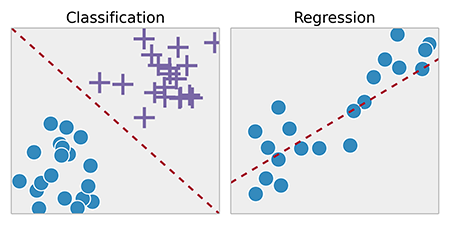
\includegraphics[width=0.8\linewidth]{images/ClassReg.png}
\end{center}
\caption{Différence entre Classification et Régression}
\label{fig:7}
\end{figure}

- \textbf{Classification :} Chaque observation ou donnée  est associée à une et une seule modalité (appelée classe/catégorie), La classification c'est le type de problème dans lequel la sortie attendu de l'algorithme est discrète c'est à dire elle est sous forme d'une catégorie ou classe.
    
    
- \textbf{Régression :} La variable de sortie de l'algorithme est quantitatif, c'est à dire elle  prend des valeurs dans un sous-domaine de l’ensemble des nombres réels. exemple: La prédiction de la rentabilité d'une compagne marketing. 


Notre problématique est la prédiction de la stratégie de récupération d'un service Web composite, c'est à dire prédire le mécanisme de récupération qui va être mis en oeuvre en cas de panne, nos données d'apprentissage sont des données générées par  un exécuteur des services Web composites vu dans l'étude précédente (Chapitre :État de l'art), qui permet de prendre la décision de choix de mécanisme de récupération, ce qui va nous permettre d'avoir un ensemble des données annotées par leur catégories de récupération. 

D'après cet analyse on peut situer notre problème de Machine Learning dans la famille des problèmes Supervisés de Classification.

\subsubsection{Les algorithmes Supervisé de Classification}

Il existe plusieurs algorithmes qui permettent la construction d'un modèle de classification, on  a sélectionne les six algorithmes les plus importants pour notre problématique de classification : 

   	
\textcolor{Orange}{\textbf{Forêt aléatoire (Randomforest) :}}

L’algorithme des forêts aléatoires ou forêt d’arbres décisionnels (Random Forest ) est un algorithme très récent (2000) pour la  classification et la régression, Random Forest utilise des stratégies de bagging c'est à dire c’est de faire la moyenne des prévisions de plusieurs modèles indépendants pour réduire la variance des prévisions d'un arbre de décision et donc l’erreur de prévision, améliorant ainsi leurs performances.

Cet algorithme est particulièrement performant pour les problématiques de prédiction, il effectue un apprentissage en parallèle sur plusieurs arbres de décision construits d'une façon aléatoire et entraînés sur des sous-ensemble de données différents, ensuite Les prédictions sont moyennées lorsque les données sont quantitatives ou utilisés pour un vote pour des données qualitatives, dans le cas des arbres de classification. L’algorithme des forêts aléatoires est connu pour être un des classifieurs les plus efficaces\cite{RF}.


\begin{figure}[H]
\begin{center}
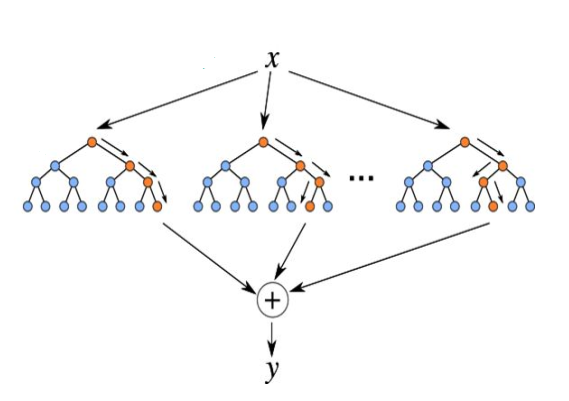
\includegraphics[width=0.8\linewidth]{images/randomforest.png}
\end{center}
\caption{Algorithme des Forêts aléatoires}
\label{fig:8}
\end{figure}

\textcolor{Orange}{\textbf{L'arbre de décision (Decision tree) : }}

Les arbres de décision sont un type d'apprentissage automatique supervisé où les données sont divisées en continu selon un certain paramètre. L'arbre peut être expliqué par deux entités, à savoir les nœuds de décision et les feuilles. Les feuilles sont les décisions ou les résultats finaux. Et les nœuds de décision sont la partie ou les données sont divisées \cite{11}.

\begin{figure}[H]
\begin{center}
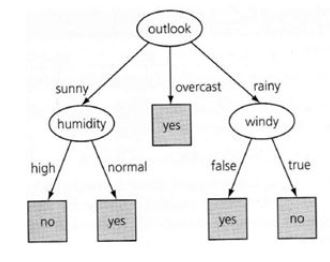
\includegraphics[width=0.8\linewidth]{images/treedecision.JPG}
\end{center}
\caption{Algorithme des arbres de décision}
\label{fig:9}
\end{figure}


\textcolor{Orange}{\textbf{Machine à vecteurs de support (Support vector machines ) : }}

Support Vector Machine (SVM) est un algorithme d'apprentissage automatique supervisé qui peut être utilisé pour les défis de classification ou de régression. Cependant, il est principalement utilisé dans les problèmes de classification. Dans cet algorithme, chaque élément de données est tracé comme un point dans un espace à n dimensions (où n est le nombre d'entités) avec la valeur de chaque entité étant la valeur d'une coordonnée particulière. Ensuite, une classification est effectuée en trouvant l'hyper-plan qui différencie très bien les deux classes.

Les vecteurs de support sont les coordonnées de l'observation individuelle. Support Vector Machine est une frontière qui sépare le mieux les deux classes (hyper-plane / ligne).


\begin{figure}[H]
\begin{center}
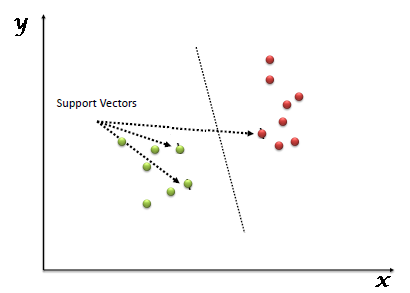
\includegraphics[width=0.8\linewidth]{images/SVM.png}
\end{center}
\caption{Algorithme de Machine à vecteurs de support}
\label{fig:10}
\end{figure}



\textcolor{Orange}{\textbf{Réseau de neurones (Neural Network) : }}

Il y a eu récemment un grand Buzz autour des "réseaux de neurones" dans le domaine de l'informatique et plus précisément dans domaine du Machine Learning, et il a attiré beaucoup d'attention de la part de nombreuses personnes.

Essentiellement, les réseaux de neurones sont composés de couches d'unités de calcul appelées neurones, avec des connexions dans les différentes couches. Ces réseaux transforment les données jusqu'à ce qu'ils puissent les classer comme une sortie. Chaque neurone multiplie une valeur initiale par un certain poids, somme les résultats avec d'autres valeurs arrivant dans le même neurone, ajuste le nombre résultant par le biais du neurone, puis normalise la sortie avec une fonction d'activation.

\begin{figure}[H]
\begin{center}
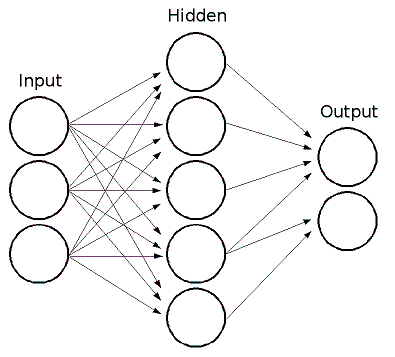
\includegraphics[width=0.7\linewidth]{images/RN.png}
\end{center}
\caption{Algorithme de Réseau de neurones}
\label{fig:11}
\end{figure}


Les réseaux de neurones se caractérise par un processus d'apprentissage itératif dans lequel les enregistrements (lignes) sont présentés au réseau une seule fois, et les poids associés aux valeurs d'entrée sont ajustés à chaque fois. Après que tous les cas sont présentés, le processus est souvent répété. Pendant cette phase d'apprentissage, le réseau s'entraîne en ajustant les poids pour prédire l'étiquette de classe correcte des échantillons d'entrée.

Les avantages des réseaux de neurones comprennent leur grande tolérance aux données bruitées, ainsi que leur capacité à classer les modèles sur lesquels ils n'ont pas été formés.


\textcolor{Orange}{\textbf{Les K plus proches voisins (K-Nearest Neighbors KNN) :}}

K plus proches voisins est un algorithme d’apprentissage supervisé. En abrégé k-NN ou KNN.
Le fonctionnement de cet algorithme se base sur un ensemble de données d'apprentissage constituée de N couples «entrée-sortie». Pour estimer la sortie associée à une nouvelle entrée x, l'algorithme des k plus proches voisins se base sur la mesure de similarité, et prend en compte (de façon identique) les k échantillons d'apprentissage dont l’entrée est la plus proche de la nouvelle entrée x, selon une distance à définir.


\begin{figure}[H]
\begin{center}
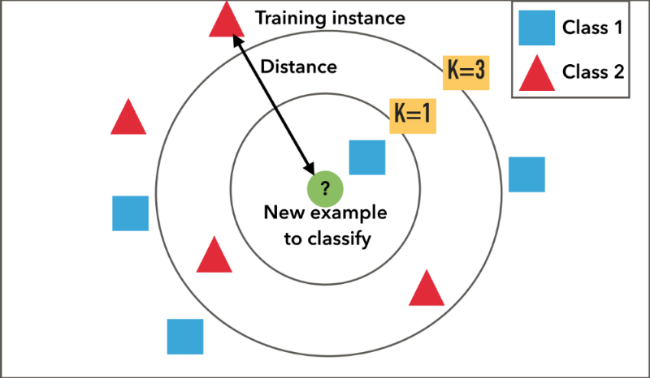
\includegraphics[width=0.8\linewidth]{images/KNN.png}
\end{center}
\caption{Classification par KNN}
\label{fig:12}
\end{figure}


Par exemple, dans un problème de classification, on retiendra la classe la plus représentée parmi les k sorties associées aux k entrées les plus proches de la nouvelle entrée x.

\textcolor{Orange}{\textbf{Classification naïve bayésienne (Naive Bayes Classification) : }}
    
L'algorithme de naïve Bayes est un algorithme de classification supervisée qui se base sur le théorème de Bayes. Ce dernier est considéré comme un résultat de base en théorie des probabilités. Ce théorème est fondé sur les probabilités conditionnelles qui consiste à savoir la probabilité qu'un événement se produise sachant qu'un autre événement s’est déjà produit.


La classification Multiple de Naive Bayes,  calcule le résultat en se basant sur plusieurs variables. L’application du théorème de Bayes sur plusieurs variables rend le calcul complexe. Pour contourner cela, une approche consiste à prendre en considération ces variables indépendamment les unes des autres. Il s’agit d’une hypothèse forte.

Généralement, les variables prédictives sont liées entre elles. Le terme “naïve” vient du fait qu’on suppose cette indépendance des variables.\cite{NB}


\section{Construction du modèle de prédiction}

Cette partie consiste l'exécution des algorithmes de classification cités dans la section précédente, afin de pouvoir choisir l'algorithme le plus performant pour notre échantillon de données. 

Pour l'exécution de ces algorithmes, on utilisera  Pentaho, l'outil utilisé précédemment dans l'intégration des données, qui offre une extension dédiée au data Mining. 

Après l'exécution de chaque algorithme de Machine Learning, on est censé choisir un outil de mesure de performance, pour qu'on puisse choisir un ou les algorithmes les plus performants pour notre problématique. 

\subsection{WEKA}

Pentaho Data Mining, est basé sur le projet WEKA, c'est un ensemble complet d'outils pour l'apprentissage automatique et l'exploration de données. Sa large gamme de règles de classification, de régression, d'association et de clustering peut être utilisée pour mieux comprendre l'activité et être exploitée pour améliorer les performances futures grâce à l'analyse prédictive \cite{10}.

WEKA est un outil qui permet d'exécuter des algorithmes de Machine Learning sur un ensemble de données. Il est ainsi possible d’isoler des populations ou d’extraire des règles à partir des données contenues dans un entrepôt de données. 

WEKA est présenté sous forme d’une application indépendante, disposant d’une interface utilisateur graphique ou en ligne de commande \cite{9}.


\begin{figure}[H]
\begin{center}
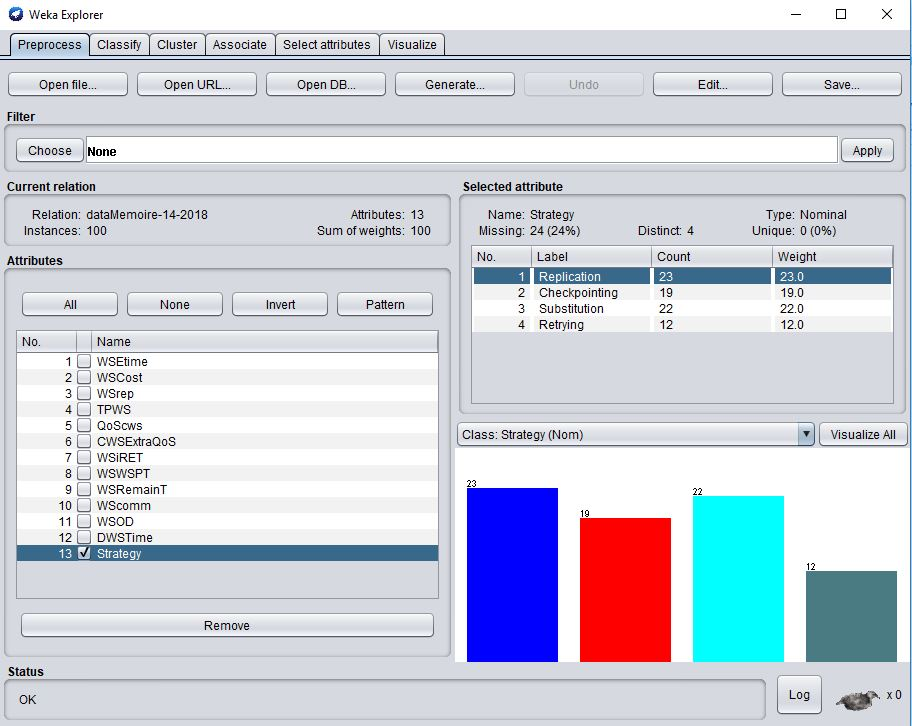
\includegraphics[width=1\linewidth]{images/weka1.JPG}
\end{center}
\caption{Importation des données sur Weka}
\label{fig:13}
\end{figure}

Après l'importation des données dans WEKA, ce dernier offre a travers les six onglets au-dessus les différentes étapes du processus d'apprentissage, soit un apprentissage supervisé ou non. 

Le premier onglet "Preprocess" permet la saisie des données, l'analyse et la sélection des attributs. 

Une fois les données sont chargées, une liste des attributs apparaît à gauche de la fenêtre, et un certain nombre de statistiques à droite qui présentent les valeurs maximales, minimales et moyennes.
En bas de la fenêtre, Weka présente un histogramme qui indique la répartition des exemples pour l'attribut sélectionné, la couleur indique la proportion d’éléments de chaque classe dans chaque colonne. On peux visualiser tous les histogrammes en même temps, cela nous donne une idée sur la répartition des données par classe (Stratégie de récupération) et par attribut. 

La figure ci-dessus, présente l'histogramme de répartition par la classe "Strategy", qui se compose de quatre catégories (Replication, Checkpointing, Substitution, Retrying), et qui sont présentées par quatre couleurs différentes. 

\subsubsection{Classification WEKA}

Le deuxième onglet de Weka "Classify" permet d'accéder à la fenêtre où on peut exécuter les algorithmes de classification sur nos données afin de construire notre modèle, c'est la partie dans laquelle on va tester tous nos algorithmes cités dans la section précédente.

\begin{figure}[H]
\begin{center}
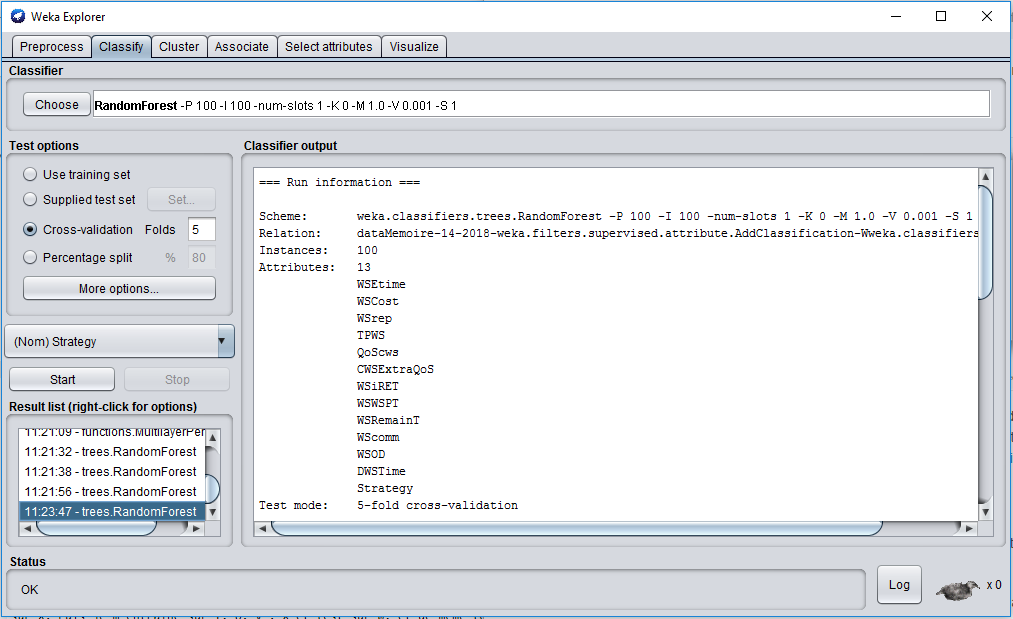
\includegraphics[width=1\linewidth]{images/wekaClassifier.PNG}
\end{center}
\caption{WEKA Classifier}
\label{fig:14}
\end{figure}

Dans cet étape on va exécuter tous les algorithmes précédents on choisissant une option de test pour les données, pour qu'on puisse faire une comparaison qui se base sur une mesure de performance qui sera à la fois la mesure de précision et la matrice de confusion. 

\textbf{Options de Test :}


\begin{figure}[H]
\begin{center}
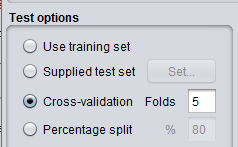
\includegraphics[width=0.5\linewidth]{images/TestOptions.PNG}
\end{center}
\caption{Options de Test WEKA}
\label{fig:15}
\end{figure}


Généralement, quand on utilise un algorithme d'apprentissage automatique, il faut en avoir des données d'apprentissage et des données de test. afin de permettre a WEKA de faire le test après la phase d'apprentissage, il faut l'informer a travers des options de la procédure à suivre concernant les données de test qui seront utilisées.

WEKA dispose de quatre options de test : 

\begin{itemize}

\item \textbf{Use training set : }  Signifie que le test sera sur les mêmes données qu'on a exploitées dans l'apprentissage. 

Généralement, cette option n'est pas performante pour une vrai évaluation d'algorithme, car on reste sur les même données.
Elle est utilisée que lorsqu'on dispose de toutes les données et qu'on souhaite créer un modèle descriptif plutôt qu'un modèle prédictif. Parce qu'il y a toutes les données, et on aura pas besoin de faire de nouvelles prédictions. Ce qui n'est pas le cas pour notre problématique de prédiction, donc cette option ne sera pas prise en compte dans notre étude.


\item \textbf{Supplied test set : }   Il s'agit d'un fichier externe qui contient des données de même modèle que les données d'apprentissage, sauf qu'elles ne sont pas annotées.

Cette Option est pratique lorsque les données sont très volumineuses, et pas un besoin de tout les exploiter pour former un modèle.

Nous disposons dans un premier temps d'un échantillon de données qui est limité et que l'on utilise pour l'apprentissage. L'option Supplied test Set n'est pas convenable avec nos conditions.


\item \textbf{Percentage split : } fractionne les données et sépare un x\% des données pour l'apprentissage et le reste pour les tests. C'est utile quand l'algorithme est lent.
Excellent à utiliser pour avoir une idée rapide de la performance d'un modèle. Il n'est pas utilisé pour prendre des décisions, du coup il se sera pas utile pour notre étude.

\item \textbf{Cross-validation : }C'est un processus qui divise l'échantillon d'apprentissage original en K échantillons, le K est nombre précisé dans "Folds".  
En prenons Folds = 5, les données seront divisées en 5 sous échantillons, et pendant 5 itérations, on prend 4 sous échantillons pour apprentissage et un seul pour le test \cite{7}.

C'est la méthode d’estimation de fiabilité de test la plus utilisée. Elle fournit généralement une estimation plus précise de la performance que les autres techniques. Ne doit pas être utilisé lorsqu'il y a une très grande quantité de données. Les valeurs communes pour k sont 5 et 10, selon la taille de l'ensemble de données. Donc la validation croisée répondra bien a notre besoin pour avoir une estimation plus précise. 

\end{itemize}

D'après le comparatif d'options fait ci-dessus, on constate que l'option la plus adaptée pour notre objectif et pour notre nature de données sera la validation croisée, en prenant un  K=5 car a priori on a pas une grande masse de données.

\subsection{Mesure de performance}


Le but de la modélisation prédictive de la stratégie de récupération des services Web composites est de créer un modèle qui fonctionne le mieux dans une situation que nous ne comprenons pas complètement, avec des nouvelles données et informations concernant les QoS des Services Web qui sont inconnues. Nous devons utiliser des techniques statistiques puissantes pour estimer au mieux la performance du modèle.

WEKA fourni un résumé des performances lorsqu'on évalue un modèle, dans l'onglet "Classifier" après avoir cliquer sur le bouton "Start", les résultats sont présentés dans le volet "Classifier Output".

Ce volet contient beaucoup d'informations, notamment:

- Les informations d'exécution telles que l'algorithme et sa configuration, l'ensemble de données et ses propriétés ainsi que l'option de test.

- Les détails du modèle construit, le cas échéant.

- Le résumé de la performance, y compris un ensemble de mesures différentes.

Lorsqu'on évalue un algorithme de Machine Learning sur un problème de classification, On reçoit une grande quantité d'informations sur les performances à assimiler.


\begin{figure}[H]
\begin{center}
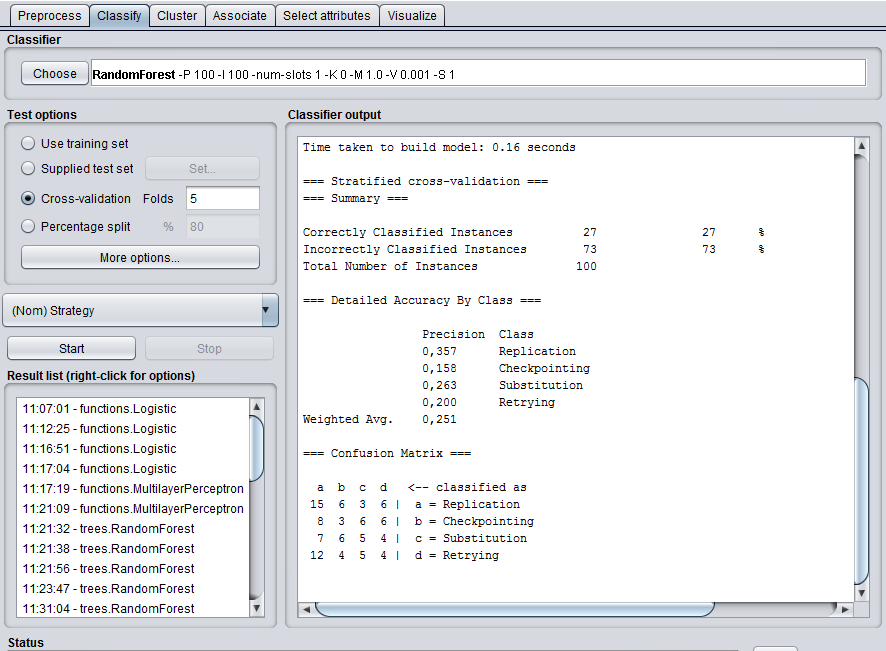
\includegraphics[width=1\linewidth]{images/summaryPerf.PNG}
\end{center}
\caption{Résumé des performances de classification pour un modèle}
\label{fig:16}
\end{figure}

Pour la classification, il existe trois aspects principaux dans le bilan de performance du modèle:

\begin{enumerate}
\item La précision de classification - Classification accuracy - : C'est le ratio entre le nombre de prédictions correctes et toutes les prédictions faites, souvent présenté sous forme d'un pourcentage où 100\% est le meilleur qu'un algorithme peut atteindre.

\item La précision par classe - Accuracy by class - : Représente le taux vrai-positif et faux-positif pour la prédictions de chaque classe, ces pourcentage peuvent donner une idée sur la répartition des classes. Cela peut aider à interpréter les résultats pour savoir si la prédiction d'une classe est plus importante que la prédiction d'une autre.

\item Matrice de confusion - Confusion matrix - : Un tableau montrant le nombre de prédictions pour chaque classe par rapport au nombre d'instances qui appartiennent réellement à cette classe. Ceci est très utile pour avoir un aperçu des types d'erreurs que l'algorithme a faites.

\end{enumerate}

Notre approche a pris en considération les trois métriques de performance pour évaluer les algorithmes de classification de stratégie de récupération des Services Web Composites. 

\subsection{Évaluation expérimentale}

Dans cette section, on présente la mise en oeuvre les algorithmes de classification des stratégies de récupération cités dans la section précédentes en mesurant leurs performances à travers les trois métriques de classification disponible sur WEKA.
L'objectif c'est la récupération et la comparaison des performances de chaque algorithme pour en pouvoir choisir le modèle le plus précis.

Les résultats obtenus dans cette évaluation sont des hypothèses, puisque les données sur lesquelles nous nous sommes basées sont des données générées aléatoirement.

WEKA mis en disposition plusieurs algorithmes de Machine Learning, algorithme de classification, régression, Cluster ...

\begin{figure}[H]
\begin{center}
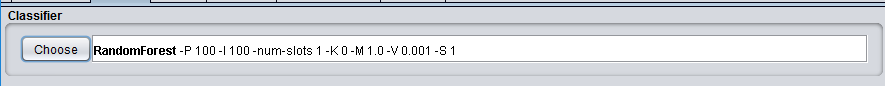
\includegraphics[width=1\linewidth]{images/algorithme.PNG}
\end{center}
\caption{Choix de l'algorithme de classification}
\label{fig:17}
\end{figure}

Tous les algorithmes présentés dans la section "Algorithme de classification"  (Random forest, Decision tree, Support vector machines, neural network, KNN, Naive Bayes) sont disponibles dans WEKA en cliquant sur le bouton "choose". L'objectif c'est de les pouvoir exécuter et récupérer leurs performances.

\subsubsection{Forêt aléatoire (Random forest) :}

Après l'exécution de l'algorithme Random forest sur notre échantillon de données on a eu les résultats montrés dans la figure ci-dessous, avec une précision de 27\%.

\begin{figure}[H]
\begin{center}
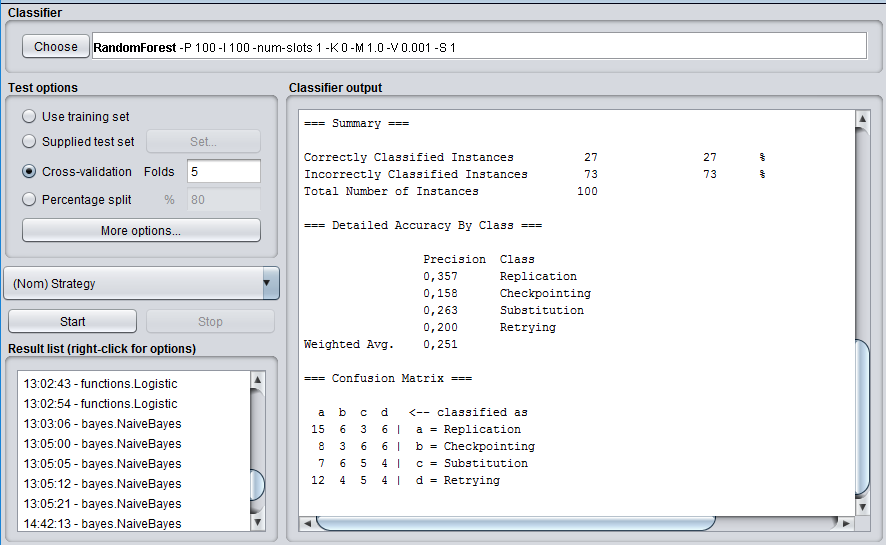
\includegraphics[width=0.8\linewidth]{images/perfRF.PNG}
\end{center}
\caption{Performance de Random Forest}
\label{fig:166}
\end{figure}


\subsubsection{L'arbre de décision (Decision Tree) :}

L'algorithme Decision Tree, a donné 27\% de précision après son exécution.

\begin{figure}[H]
\begin{center}
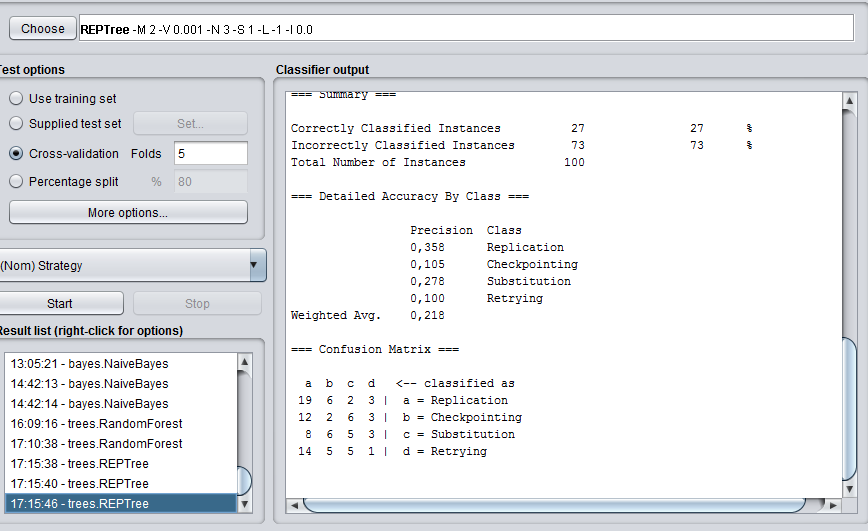
\includegraphics[width=0.8\linewidth]{images/perfDecTree.PNG}
\end{center}
\caption{Performance de Decision Tree}
\label{fig:27}
\end{figure}


\subsubsection{Machine à vecteurs de support (Support vector Machine) :}

Après l'exécution de l'algorithme Support sur notre échantillon de données on a eu un résultat de 31\% de précision.

\begin{figure}[H]
\begin{center}
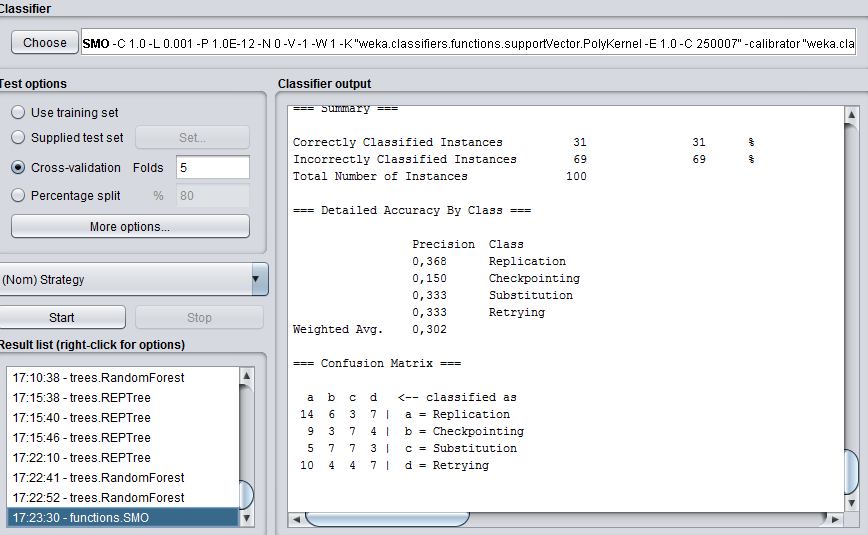
\includegraphics[width=0.8\linewidth]{images/perfSMO.PNG}
\end{center}
\caption{Performance de Support vector Machine }
\label{fig:18}
\end{figure}

\subsubsection{Réseau de neurones (Neural Network) :}

Après l'exécution de l'algorithme Neural Network sur notre échantillon de données on a eu les résultats montrés dans la figure ci-dessous, avec une précision de 30\%.

\begin{figure}[H]
\begin{center}
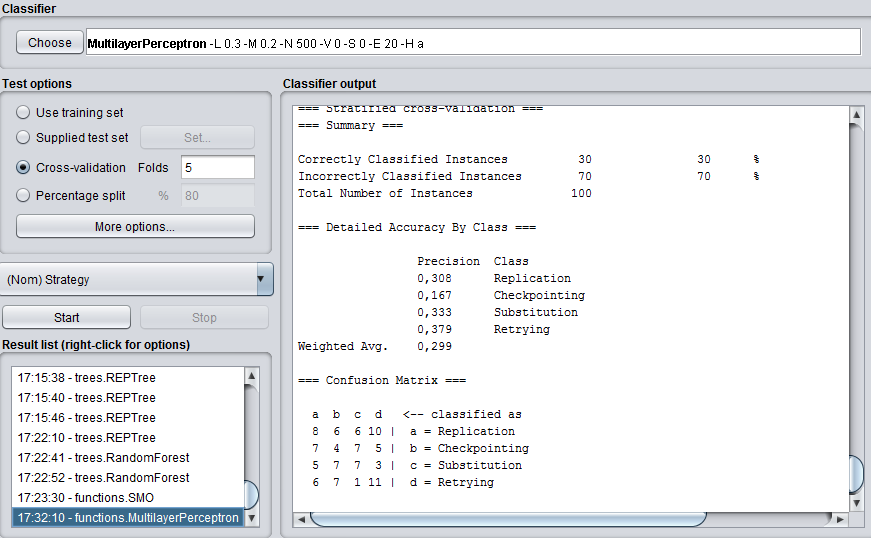
\includegraphics[width=0.8\linewidth]{images/perfNN.PNG}
\end{center}
\caption{Performance de Neural Network}
\label{fig:19}
\end{figure}

\subsubsection{Les k plus proches voisins (K-Nearest Neighbors KNN)}
Après l'exécution de l'algorithme KNN sur notre échantillon de données on a eu un résultat de 22\% de précision.

\begin{figure}[H]
\begin{center}
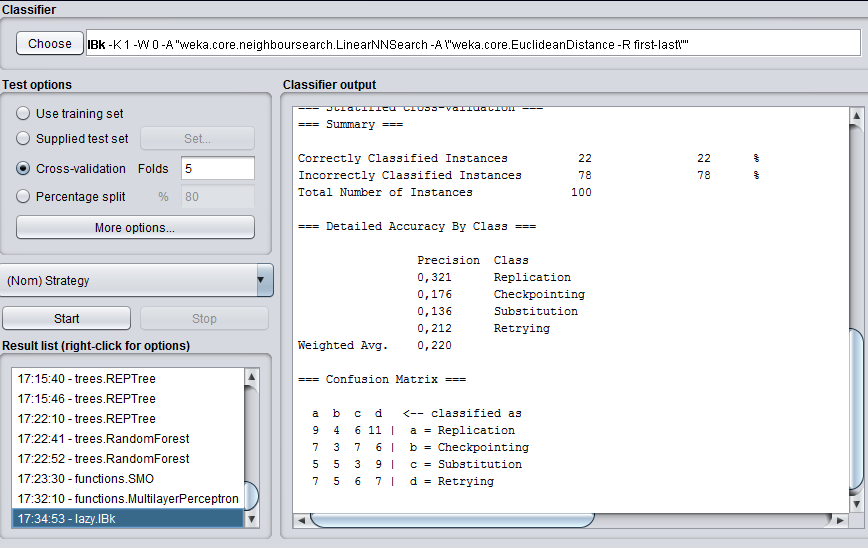
\includegraphics[width=0.8\linewidth]{images/perfKNN.PNG}
\end{center}
\caption{Performance de KNN}
\label{fig:20}
\end{figure}

\subsubsection{Naive Bayes}

L'algorithme Decision Tree, a donné 32\% de précision après son exécution.

\begin{figure}[H]
\begin{center}
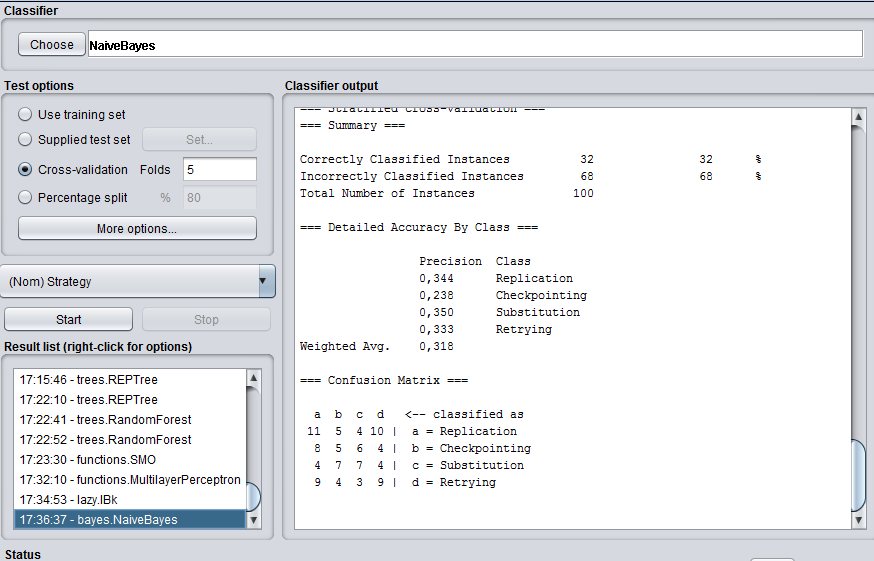
\includegraphics[width=0.8\linewidth]{images/perfNB.PNG}
\end{center}
\caption{Performance de Naive Bayes}
\label{fig:21}
\end{figure}

\textcolor{Orange}{\textbf{Résultat :}} 

D'après les résultats obtenus après l'exécution de chaque algorithme on a résumé les précisions dans le tableau suivant : 

\begin{figure}[H]
\begin{center}
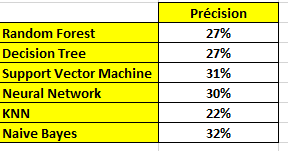
\includegraphics[width=0.6\linewidth]{images/stat.PNG}
\end{center}
\caption{Tableau concluant la précision des algorithme}
\label{fig:22}
\end{figure}

Les résultats montrent que les modèles les plus précis sont ceux obtenus par l'algorithme de Naive Bayes et  de Support Vector Machine avec une précision de 32\% et 31\%.

Cela reste une hypothèse comme cité au par avant car les données sur lesquelles on se base sont des données temporaires, qui sont générées d'une manière aléatoire a priori pour décrire le processus de prédiction de la stratégie de récupération. 

